%\documentclass[titlepage]{jsarticle}

%\usepackage[dvipdfmx]{graphicx}

%数式用パッケージ
%\usepackage{amsmath, amssymb}
%\usepackage{mathtools}
%\usepackage{cancel}
%\usepackage{cases}
%\usepackage{bm}
%\usepackage{array,booktabs}
%\usepackage{float}

%\usepackage{subcaption}

%ファインマングラフ用パッケージ
%\usepackage{feynmf}



%\graphicspath{{./figure/}}

%\begin{document}

%%%%%%%%%%%%%%%%%%%池満パート開始%%%%%%%%%%%%%%%%%%%
\section{プラスチックシンチレータで取得したデータの解析と考察}

プラスチックシンチレータのデータの解析では波形解析やイベント選択について異なる2つの解析手法を適用し,それぞれで寿命と$g$ 因子の2つを求めた.以下ではそれぞれの解析手法に解析A, Bと名付け解説し,最後にそれらの両方の結果をまとめる.
 
\subsection{解析手法A}
\subsubsection{解析の流れ}
プラスチックシンチレータ(以下,PS )検出器を用いて取得したデータを以下の方法で解析し,寿命,$g$ 因子,エネルギー分布を求めた.
\begin{enumerate}
\item イベントディスプレイから,初めの100~ns (50~Sample) の間は信号が来ていないことを確認し,0~-~100~ns のデータの平均値をとってそれをbaseline とした.
\item 信号のしきい値 (threshold) の決定
\begin{itemize}
\item 宇宙線を用いた予備実験の結果から,12~MeV のエネルギーに対応する信号のピーク値を求めた.(表~\ref{12MeVpeak})%宇宙線を用いた予備実験の説明は?? 12MeVがMIPがPSの厚さを通った時に落とすエネルギーである説明.
\item そのピーク値から,各チャンネルごとのthreshold を以下の値に決めた.ただし,本実験ではチャンネル~4 でフィンガーカウンターの信号を取ったので,そのthreshold は表~\ref{12MeVpeak} と関係無くイベントディスプレイを元に適当な値 (20~mV) に決めた.
\item 寿命測定と$g$ 因子測定用には全チャンネルとも4~MeV 相当とした.4~MeV 相当にした理由については後述する.
\item エネルギー測定用には,1 層目にのみ4~MeV 相当のthreshold を設けた.2 層目以降にthreshold を設けなかったのは,4~MeV 相当のthreshold を超えるエネルギーを持つイベントを全て取るためである.
\end{itemize}
\item 各チャンネルごとで,threshold を越えた時間を信号の時間 (peaktime) とした.
\item イベントディスプレイからおおよその信号の時間幅を決め,信号が検出されてから次の信号を検出するようになるまでのveto 時間を40~ns にした.
\item peaktime から40~ns の間のデータを足すことで信号のcharge を求めた.
\item 寿命と$g$ 因子について
\begin{itemize}
\item 各層の両側のチャンネルの信号のコインシデンスを取った.ただし,3 層目は片側のみの信号である.
\item ここで,コインシデンスの条件は互いのpeaktime が10~ns よりも近いものとした.
\item 寿命測定ではフィンガーカウンターを要求せずに層ごとのコインシデンスのみをとった.
\item $g$ 因子測定では立体角を制限するために,層ごとだけでなくフィンガーカウンターとのコインシデンスを要求した.
\end{itemize}
\item エネルギーについて
\begin{itemize}
\item 予備実験のデータから,各チャンネルごとにキャリブレーションをした.
\item 各層のエネルギーとして,1, 2, 4 層目では両側のチャンネルのエネルギーの平均を取り,3 層目では片方のチャンネルのエネルギーを使用した.
\item フィンガーカウンターと1 層目の両側のチャンネルの信号のコインシデンスをとり,そのときの全層のエネルギーの和を求めた.
\item そのエネルギーにフィンガーカウンターで落とすエネルギーとして1.5~MeV を足した.
\item フィンガーカウンターとのコインシデンスを取ったのは,検出器の中心に入った$e^{+}$ の信号のみを選択するためである.高エネルギーの$e^{+}$ が入射すると検出器との相互作用によって電磁シャワーが生じる.このシャワー中の粒子が外に漏れ出ると,検出されるエネルギーは実際の$e^{+}$ のエネルギーよりも低い値になる.$e^{+}$ の入射位置が検出器の端にある場合,検出器中央に入射する場合よりも電磁シャワー中の電子や陽電子が検出器の外に漏れやすい.以上のことから$e^{+}$ が検出器の中央に入射したイベントのみを解析に用いるべきだと考え,フィンガーカウンターとのコインシデンスを要求した.
\end{itemize}
\end{enumerate}

寿命と$g$ 因子の解析に関して,解析方法B との主な違いは次の3 点である.
\begin{itemize}
\item threshold の値を各チャンネル毎に変えていること
\item 信号検出後にveto 時間を設けていること
\item 層間およびフィンガーカウンターとコインシデンスをとっていること
\end{itemize}
  
\begin{table}[h]
\caption{12~MeV に対応するchargeをもつ信号のピーク}
\label{12MeVpeak}
\centering
\begin{tabular}{cc}\toprule
PMT 名&ピーク値~[mV] \\ \hline
チャンネル0(あけみ) & 110 $\pm$ 21 \\
チャンネル1(勝太郎) & 145 $\pm$ 25 \\
チャンネル2(畑さん) & 160 $\pm$ 28 \\
チャンネル3(紗智子) & 112 $\pm$ 22 \\
チャンネル4(蘭) & 140 $\pm$ 23 \\
チャンネル5(矢部) & 161 $\pm$ 28 \\
チャンネル6(政子) & 105 $\pm$ 21 \\
チャンネル7(王) & 140 $\pm$ 25 \\ \bottomrule
\end{tabular}
\end{table}

\subsubsection{信号検出のthreshold 値について}
信号検出時のthreshold の値の判断理由について触れておく.Threshold の値を1~MeV 相当から6~MeV 相当まで変化させて寿命を求めると,threshold が1~MeV 相当から高くなるにつれて寿命は短くなり,4~MeV 相当以上のときに誤差の範囲で一定の値になった.このことから3~MeV 相当以下のthreshold では低エネルギーのノイズを信号として処理していると考えた.よって,threshold の値には4~MeV 相当の電圧値が妥当だと考えた.

\begin{table}[h]
 \caption{threshold 値を変更したときの寿命(ns)}
 \label{PS_decide_threshold}
 \centering
 \begin{tabular}{ccccc}\toprule
  threshold 値 & 1層 & 1+2層 & 1〜3層 & 1〜4層 \\ \hline
  1~MeV& $2236.4\pm 6.5$ & $2283.4\pm 9.4$ & $2292\pm 12$ & $2296\pm 24$ \\
  2~MeV& $2223.7\pm 7.2$ & $2238.7\pm 9.6$ & $2241\pm 13$ & $2209\pm 28$ \\
  3~MeV& $2227.6\pm 7.5$ & $2229.6\pm 9.9$ & $2227\pm 14$ & $2180\pm 31$ \\
  4~MeV& $2223.7\pm 7.7$ & $2225  \pm 10 $ & $2218\pm 15$ & $2149\pm 35$ \\
  5~MeV& $2223.3\pm 8.0$ & $2223  \pm 11 $ & $2204\pm 16$ & $2157\pm 42$ \\
  6~MeV& $2217.4\pm 8.4$ & $2218  \pm 12 $ & $2197\pm 17$ & $2165\pm 51$ \\ \bottomrule
 \end{tabular}

\end{table}

\subsubsection{得られた崩壊曲線とフィッティングの結果}
図~\ref{lt_layercoin} は,磁場なし標的を用いたときのミューオンの崩壊曲線である.それを次の$f_{\mathrm{life}}(t)$ でフィッティングした結果が図~\ref{lt_layercoin_fit} である.
\[f_{\mathrm{life}}(t) = \exp[-(t+A)/\tau]\]

また,図~\ref{g_layercoin} は磁場あり標的を用いたときのミューオンの崩壊曲線である.それを次の$f_{g}(t)$ でフィッティングした結果が図~\ref{g_layercoin_fit} である.
\[f_{g}(t) = \exp[-(t+A)/\tau](1+B\cos(\omega t + \delta))\]

  
フィッティングの範囲は1050~ns から7950~ns までとした. フィッティング範囲の決定方法は以下の通りである.今回使用したミューオンビームの分布はFWHM $\sim$ 100~ns ,すなわち$\sigma \sim 50~\mathrm{ns}$ のガウス分布と考えることができる.図~\ref{lt_layercoin} のヒストグラムがピーク値をとる約800~ns をガウシアンのピークだと考えて,その点から$5\sigma$ ($\sim 250~\mathrm{ns}$ )はフィッティングの対象外とした.また,ピークを検出してから40~ns のveto 時間をとるという解析方法から,8000~ns から前の40~ns 分は解析に用いることができない.以上のことからフィッティング範囲を決定した.
  
フィッティングの結果は表~\ref{fit_lt}, \ref{fit_g}のようになった.表中の誤差はフィッティングに由来する統計誤差である.また,表~\ref{fit_g} においてFC はフィンガーカウンターを表す.
  
\begin{table}[H]
\caption{寿命$\tau$ のフィッティング結果}
\label{fit_lt}
\centering
\begin{tabular}{cc}\toprule
コインシデンスを取った層& $\tau$~[ns] \\ \midrule
1 & 2223.7 $\pm$ 7.7 \\
1+2 & 2224 $\pm$ 10 \\
1+2+3 & 2217 $\pm$ 15 \\
1+2+3+4 & 2148 $\pm$ 35\\ \bottomrule
\end{tabular}
\end{table}%
  
\begin{table}[H]
\caption{$g$ 因子のフィッティング結果}
\label{fit_g}
\centering
\begin{tabular}{cccc}\toprule
コインシデンスを取った層 & $\tau$~[ns] & $\omega$~[$\times 10^{-3}$/ns] & $g$ \\ \midrule
FC + 1 & 2170.4 $\pm$ 9.1 & $ (4.621 \pm 0.012) $ & 2.0091 $\pm$ 0.0054 \\
FC + 1 + 2 & 2199 $\pm$ 13 & $ (4.614 \pm 0.011) $ & 2.0063 $\pm$ 0.0050 \\
FC + 1 + 2 + 3 & 2205 $\pm$ 18 & $ (4.594 \pm 0.013) $ & 1.9973 $\pm$ 0.0055\\
FC+ 1 + 2 + 3 + 4 & 2142 $\pm$ 45 & $ (4.649 \pm 0.024) $ & 2.021 $\pm$ 0.011 \\ \bottomrule
\end{tabular}
\end{table}%

\begin{figure}[H]
\centering
%\begin{subfigure}{\columnwidth}
%\centering
%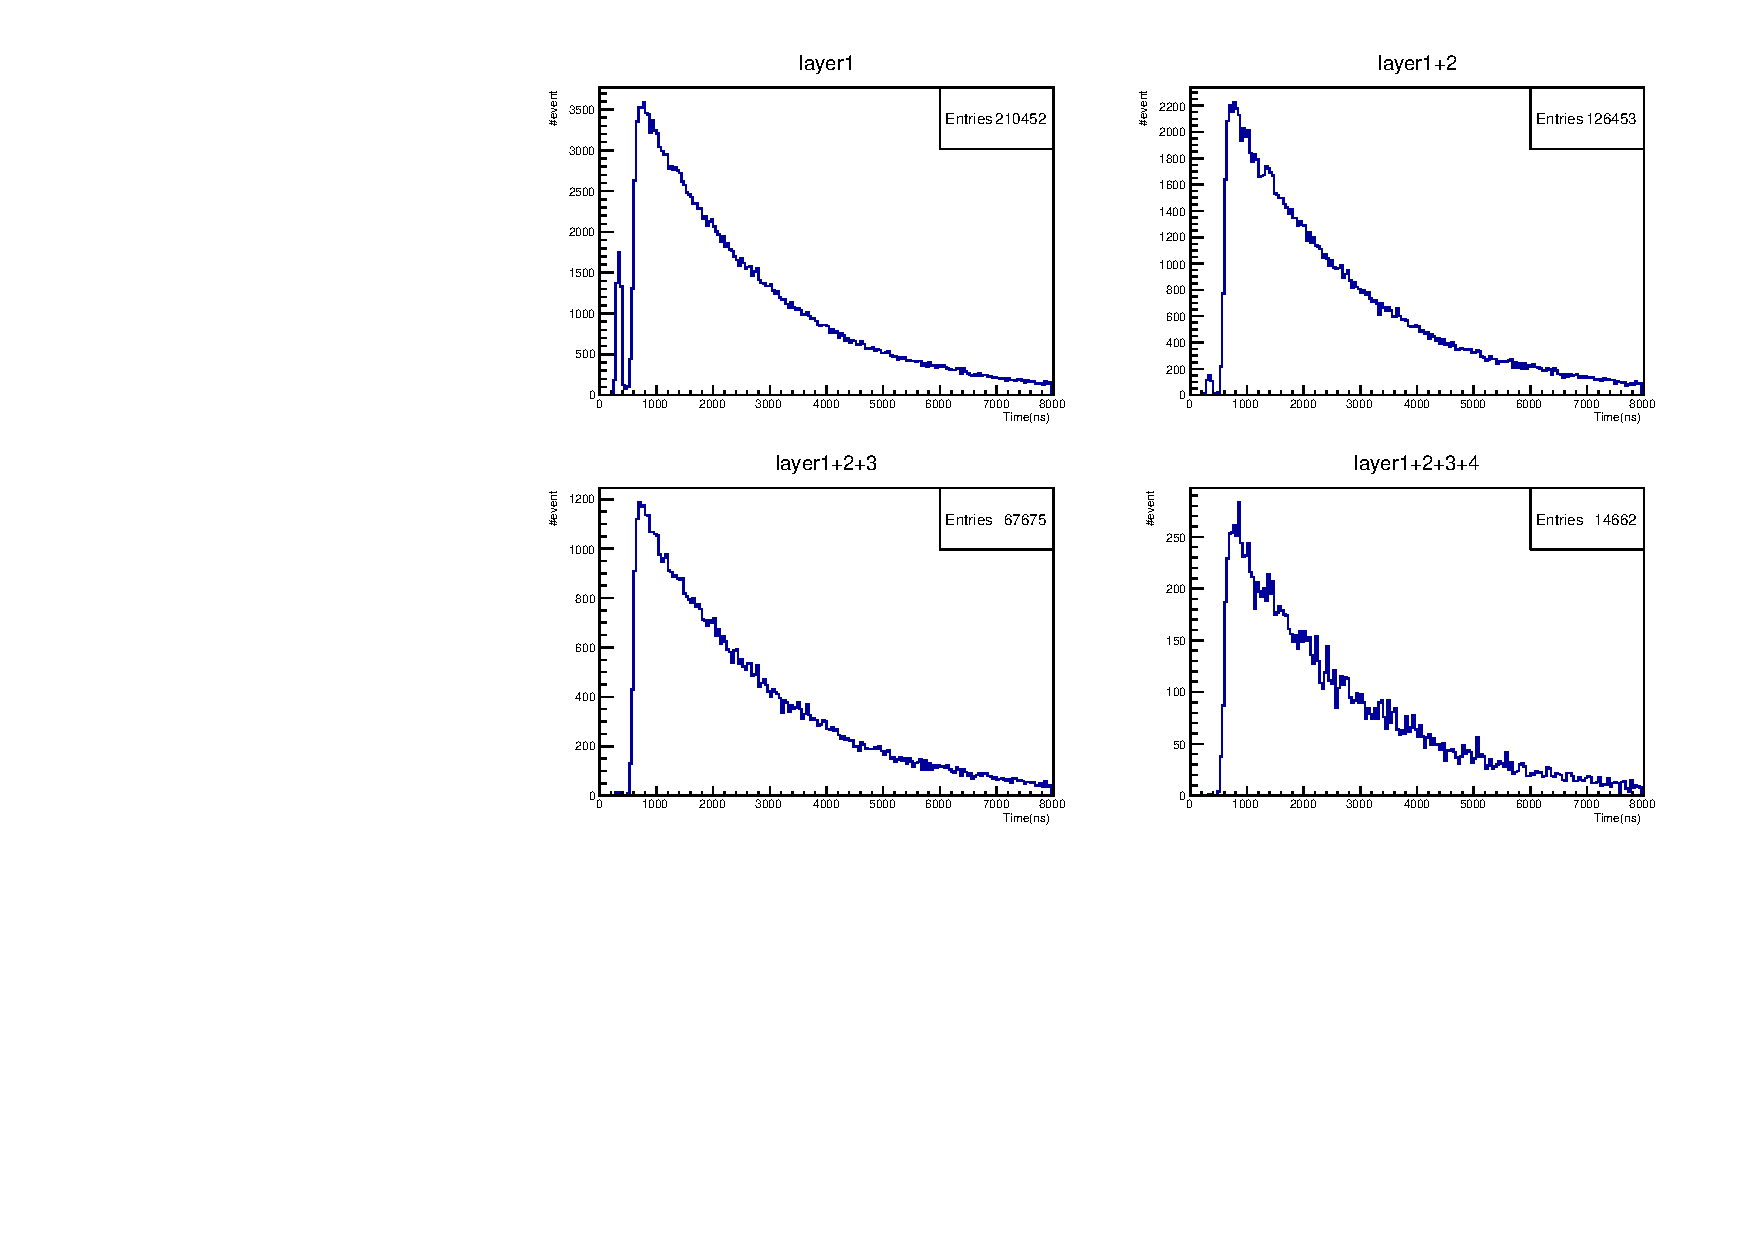
\includegraphics[height = 0.9\columnwidth , angle = -90]{figure/ikemitsu/lt_layercoin.pdf}
%\caption{層でコインシデンスを取って得られたヒストグラム(磁場なし標的)}
%\label{lt_layercoin}
%\end{subfigure}
%\begin{subfigure}{\columnwidth}
%\centering
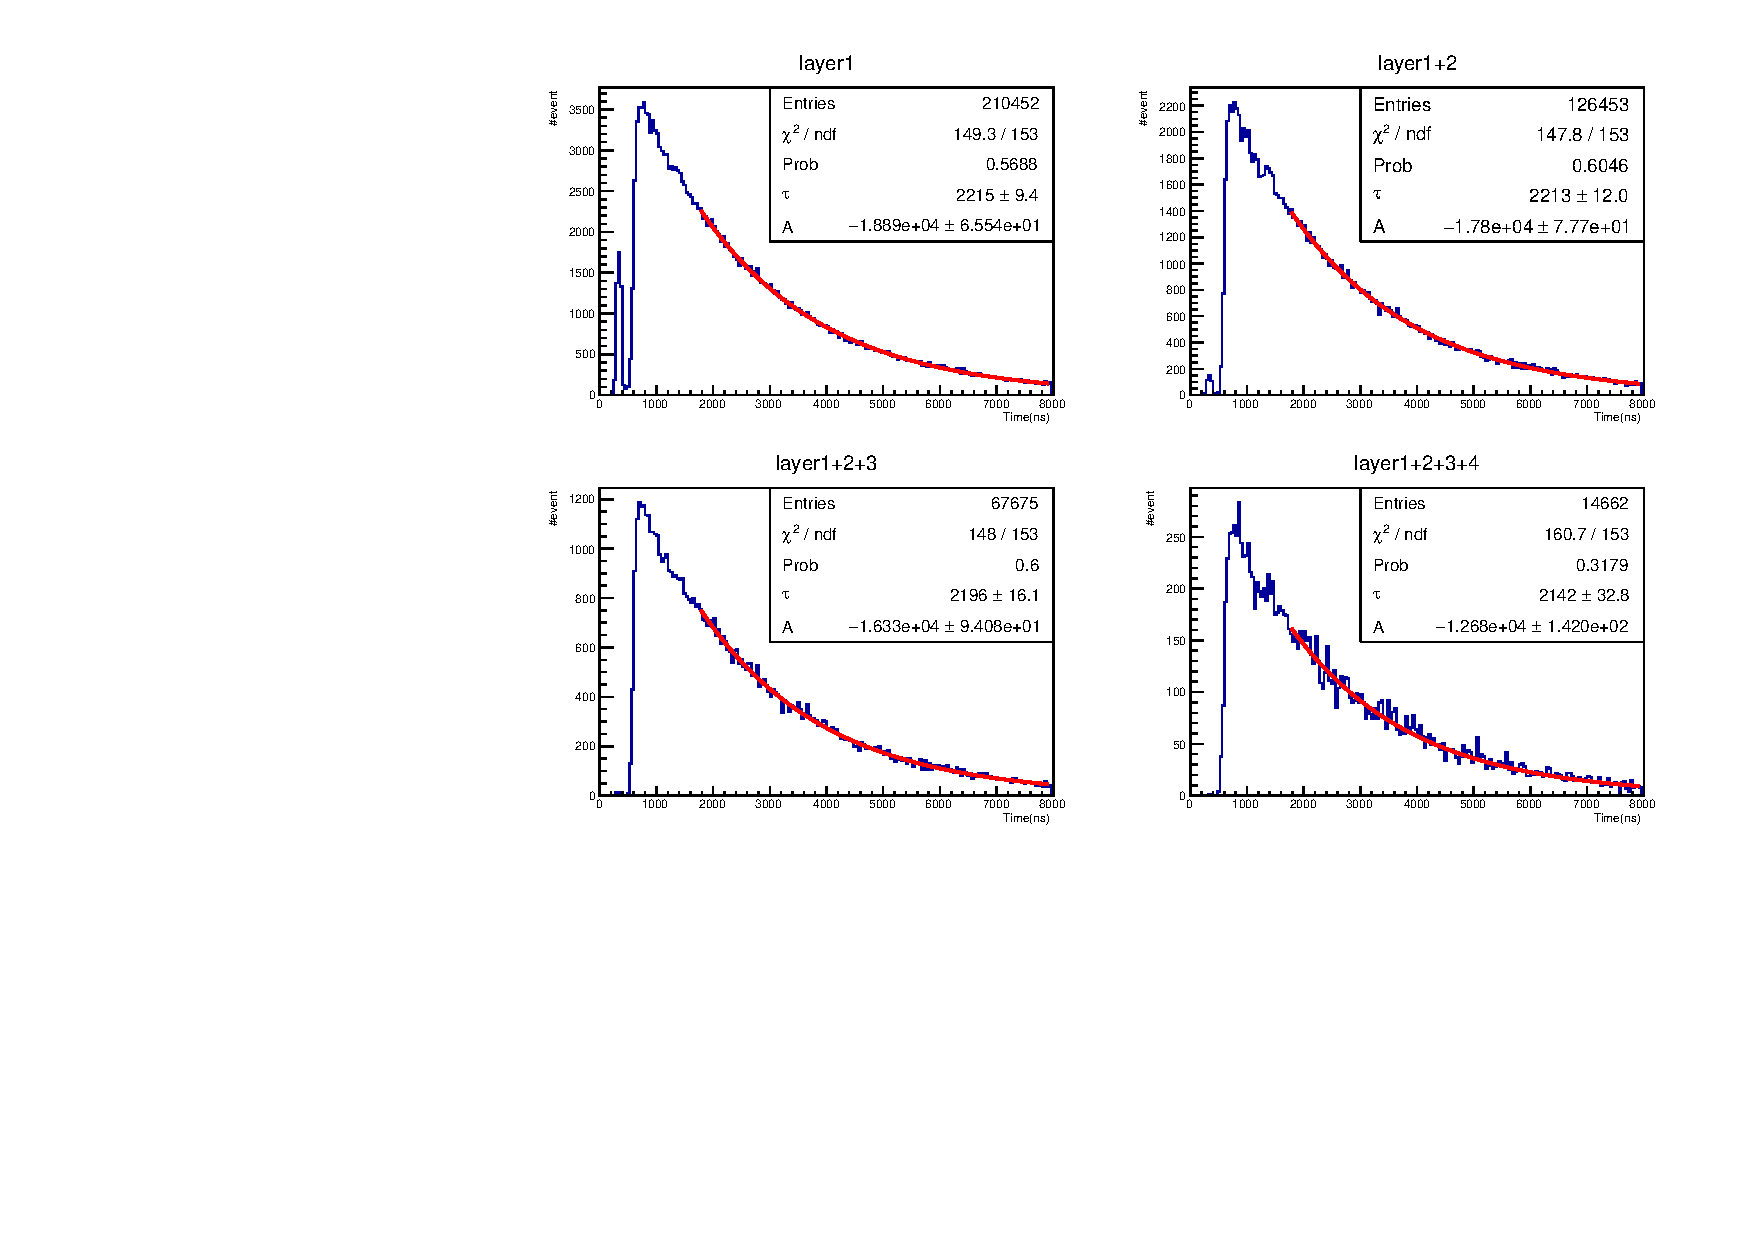
\includegraphics[height = 0.9\columnwidth , angle = -90]{figure/ikemitsu/lt_layercoin_fit.pdf}
\caption{層でコインシデンスをとったヒストグラムを$f_{\mathrm{life}}(t)$ でフィッティングした結果(磁場なし標的)}
\label{lt_layercoin_fit}
%\end{subfigure}
%\caption{フィッティングした図}
%\label{lt_layercoin_all}
\end{figure}
  
\begin{figure}[H]
\centering
%\begin{subfigure}{\columnwidth}
%\centering
%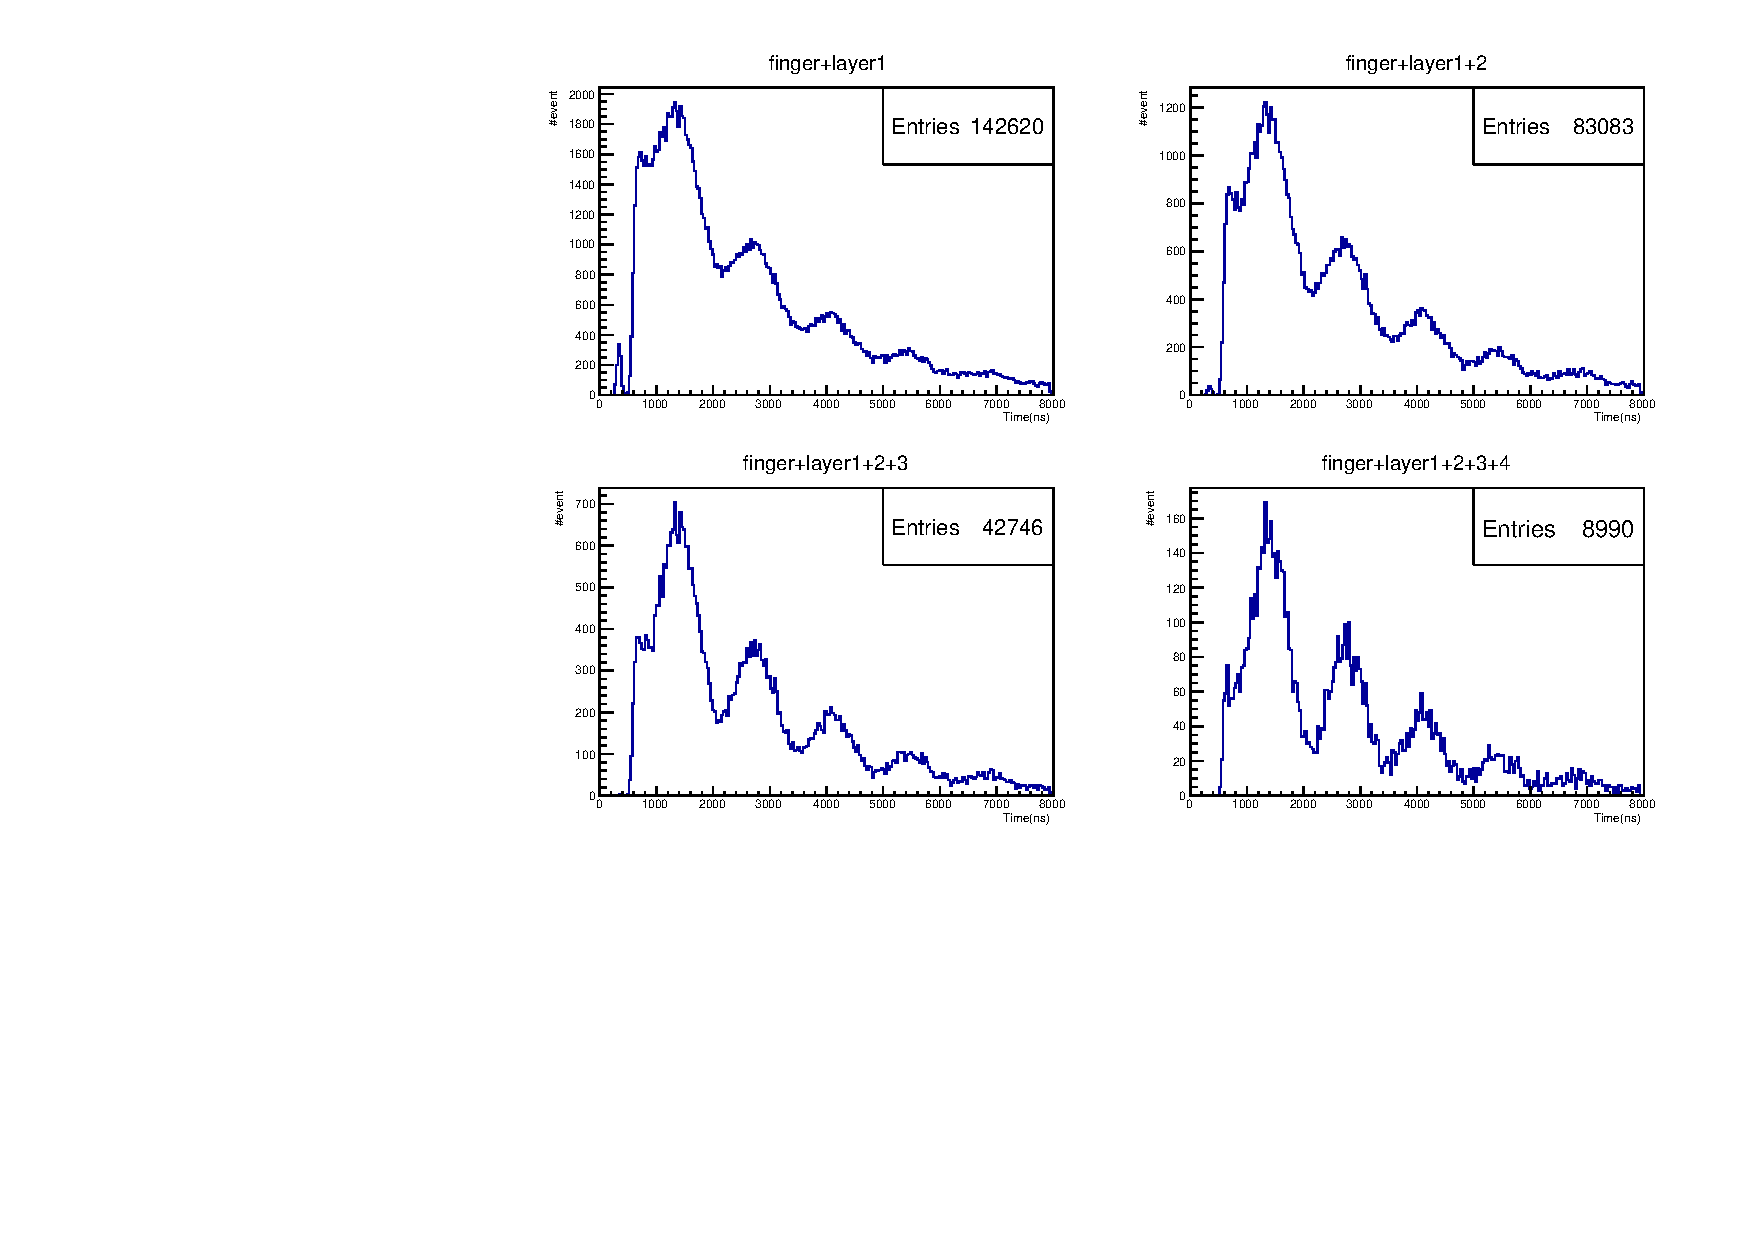
\includegraphics[height = 0.9\columnwidth , angle = -90]{figure/ikemitsu/g_layer_f_coin.pdf}
%\caption{FC と層でコインシデンスを取って得られたヒストグラム(磁場あり標的)}
%\label{g_layercoin}
%\end{subfigure}
%\begin{subfigure}{\columnwidth}
%\centering
\includegraphics[height = 0.9\columnwidth , angle = -90]{figure/ikemitsu/g_layer_f_coin_fit.pdf}
\caption{FC と層でコインシデンスをとったヒストグラムを$f_{g}(t)$ でフィッティングをした結果(磁場あり標的)}
\label{g_layercoin_fit}
%\end{subfigure}
%\caption{フィッティングした図}
%\label{g_layercoin_all}
\end{figure}

\subsubsection{フィッティング範囲の妥当性について}
上で述べたようにフィッティングの範囲は1050~ns から7950~ns としたが,この範囲の前側と後側で範囲を分けてフィッティングをすると,$\tau$ と$g$ の値は表~\ref{fitrange1} - \ref{fitrange4} のようになった.図~\ref{lt_diff} と図~\ref{g_diff} はそれぞれ,表~\ref{fitrange1}, \ref{fitrange2}, \ref{fit_lt}と表~\ref{fitrange3}, \ref{fitrange4}, \ref{fit_g}をグラフにしたものである.図中の黒丸が1050 - 7950~nsでのフィッティング結果,赤四角が1050 - 4550~nsでのフィッティング結果,青三角が4450 - 7950~nsでのフィッティング結果を表していて,左から順に1 層のみ,1, 2 層,1 - 3 層,全層でコインシデンスをとったときの値である.各層毎で3 つのフィッティング範囲の結果を比較すると,$\tau$ と$g$ の値は誤差の範囲内で一致していると言える.
  
このことから,フィッティングの範囲として1050~ns から7950~ns までは適切だと考えられる.

\begin{figure}[H]
\centering
\begin{minipage}{0.4\columnwidth}
\centering
\includegraphics[height = \columnwidth,angle=-90]{figure/ikemitsu/lt_difference.pdf}
\caption{フィッティング範囲別の寿命の値}
\label{lt_diff}
\end{minipage}
\begin{minipage}{0.4\columnwidth}
\centering
\includegraphics[height=\columnwidth,angle=-90]{figure/ikemitsu/g_differnce.pdf}
\caption{フィッティング範囲別の$g$ の値}
\label{g_diff}
\end{minipage}
\end{figure}
  
\begin{table}[H]
\centering
\begin{minipage}{0.4\columnwidth}
\caption{寿命$\tau$ (フィッティング範囲1050 - 4550~ns) }
\label{fitrange1}
\centering
\begin{tabular}{cc}\toprule
コインシデンスを取った層 & $\tau$~[ns] \\ \midrule
1 & 2233 $\pm$ 14 \\
1+2 & 2234 $\pm$ 19 \\
1+2+3 & 2249 $\pm$ 27 \\
1+2+3+4 & 2127 $\pm$ 63 \\ \bottomrule
\end{tabular}
\end{minipage}
\hspace*{5mm}
\begin{minipage}{0.4\columnwidth}
\caption{寿命$\tau$ (フィッテイング範囲4450 - 7950~ns) }
\label{fitrange2}
\centering
\begin{tabular}{cc}\toprule
コインシデンスを取った層 & $\tau$~[ns] \\ \midrule
1 & 2250 $\pm$ 32 \\
1+2 & 2238 $\pm$ 42 \\
1+2+3 & 2257 $\pm$ 61 \\
1+2+3+4 & 2013 $\pm$ 121 \\ \bottomrule
\end{tabular}
\end{minipage}
\end{table}%

\begin{table}[H]
\caption{$g$ 因子(フィッティング範囲1050 - 4550~ns }
\label{fitrange3}
\centering
\begin{tabular}{cccc}\toprule
コインシデンスを取った層 & $\tau$~[ns] & $\omega$~[$\times 10^{-3}$/ns] & $g$ \\ \midrule
FC + 1 & 2134 $\pm$ 15 & $(4.638 \pm 0.020) $ & 2.0165 $\pm$ 0.0088 \\
FC + 1 + 2 & 2185 $\pm$ 21 & $(4.612 \pm 0.020) $ & 2.0054 $\pm$ 0.0085 \\
FC + 1 + 2 + 3 & 2221 $\pm$ 32 & $(4.615 \pm 0.021) $ & 2.0068 $\pm$ 0.0093\\
FC + 1 + 2 + 3 + 4 & 2271 $\pm$ 87 & $(4.663 \pm 0.040) $ & 2.028 $\pm$ 0.018 \\ \bottomrule
\end{tabular}
\end{table}%

\begin{table}[H]
\caption{$g$ 因子(フィッティング範囲4450 - 7950~ns) }
\label{fitrange4}
\centering
\begin{tabular}{cccc}\toprule
コインシデンスを取った層 & $\tau$~[ns] & $\omega$~[$\times 10^{-3}$/ns] & $g$ \\ \midrule
FC + 1 & 2254 $\pm$ 42 & $(4.569 \pm 0.059) $ & 1.986 $\pm$ 0.026 \\
FC + 1 + 2 & 2267 $\pm$ 58 & $(4.618 \pm 0.053) $ & 2.008 $\pm$ 0.023 \\
FC + 1 + 2 + 3 & 2245 $\pm$ 86 & $(4.571 \pm 0.056) $ & 1.987 $\pm$ 0.024\\
FC + 1 + 2 + 3 + 4 & 1975 $\pm$ 186& $(4.64 \pm 0.11) $ & 2.016 $\pm$ 0.046 \\ \bottomrule
\end{tabular}
\end{table}%
%[]の中に10^-3 と書いてある場合に表内の数値も()で囲む必要があるのか?

\subsubsection{コインシデンスをとる層数による寿命の違いについて}
図~\ref{lt_diff}において,各フィッティング範囲毎に全層コインシデンス以外の3点を定数でフィッティングすると図~\ref{lt_diff_fit} のようになった.全層でコインシデンスをとったときのフィッティング結果が3 層目までの結果から明らかにずれていることがわかる.このずれが何に起因しているのかはわからなかったので,全層コインシデンスの結果は系統誤差に含めることにした.

\begin{figure}[H]
\centering
\includegraphics[height=0.6\columnwidth,angle=-90]{figure/ikemitsu/lt_difference_fit.pdf}
\caption{各フィッティング範囲毎に,全層コインシデンス以外の3 点を定数でフィッティングした結果}
\label{lt_diff_fit}
\end{figure}

$g$ 因子に関しても同様に,図~\ref{g_diff} において全層コインシデンス以外の3点を定数でフィッティングした.表~\ref{fit_lt} と表~\ref{fit_g} の値に対して行なったこれらの定数フィッティングの結果を解析手法A の結果として表~\ref{kaisekiA_matome} にまとめた.誤差は,3点の定数フィッティングの誤差を統計誤差とし,全層コインシデンスで得られた値の中央値との差を系統誤差とした.

\begin{table}[H]
\caption{解析手法A で得た寿命と$g$ 因子の結果}
\label{kaisekiA_matome}
\centering
\begin{tabular}{cc}\toprule
寿命$\tau$~[ns] & $g$ 因子 \\ \midrule
$2222.8\pm5.7 _{-75}$ & $2.0044\pm 0.0031^{+0.017}$ \\ \bottomrule
\end{tabular}
\end{table}
  
\subsubsection{エネルギー分布}
磁場なし標的を用いたときのデータから求めたエネルギーのヒストグラムは図~\ref{michel_PS}のようになった.ミューオンビームのピークと考えられる時間(800~ns 付近)から約$5\sigma$~(250~ns)の間隔を開けることでミューオンが散乱されて直接検出器に入射するイベントはほぼ無視できると考えた.したがって解析にはpeaktime が1050~ns 以降のイベントのみを使用した.
  
図~\ref{michel_PS} において横軸と縦軸の誤差として,それぞれキャリブレーション由来のエネルギー分解能と統計誤差をつけたグラフが図~\ref{michel_PS_gosa}である.
  %磁場なし標的を用いたときのデータから求めたエネルギー分布は図~\ref{michel_PS}のようになった.
  %さらに,~\ref{michel_PS}の各点において,キャリブレーションに由来するエネルギー分解能と統計誤差をそれぞれ横軸と縦軸の誤差として付けたのが図~\ref{michel_PS_gosa}である.%図の縦軸の説明 2つの図で全然スケールが違うのはなぜ?
\begin{figure}[H]
\centering
\begin{minipage}{0.4\columnwidth}
\centering
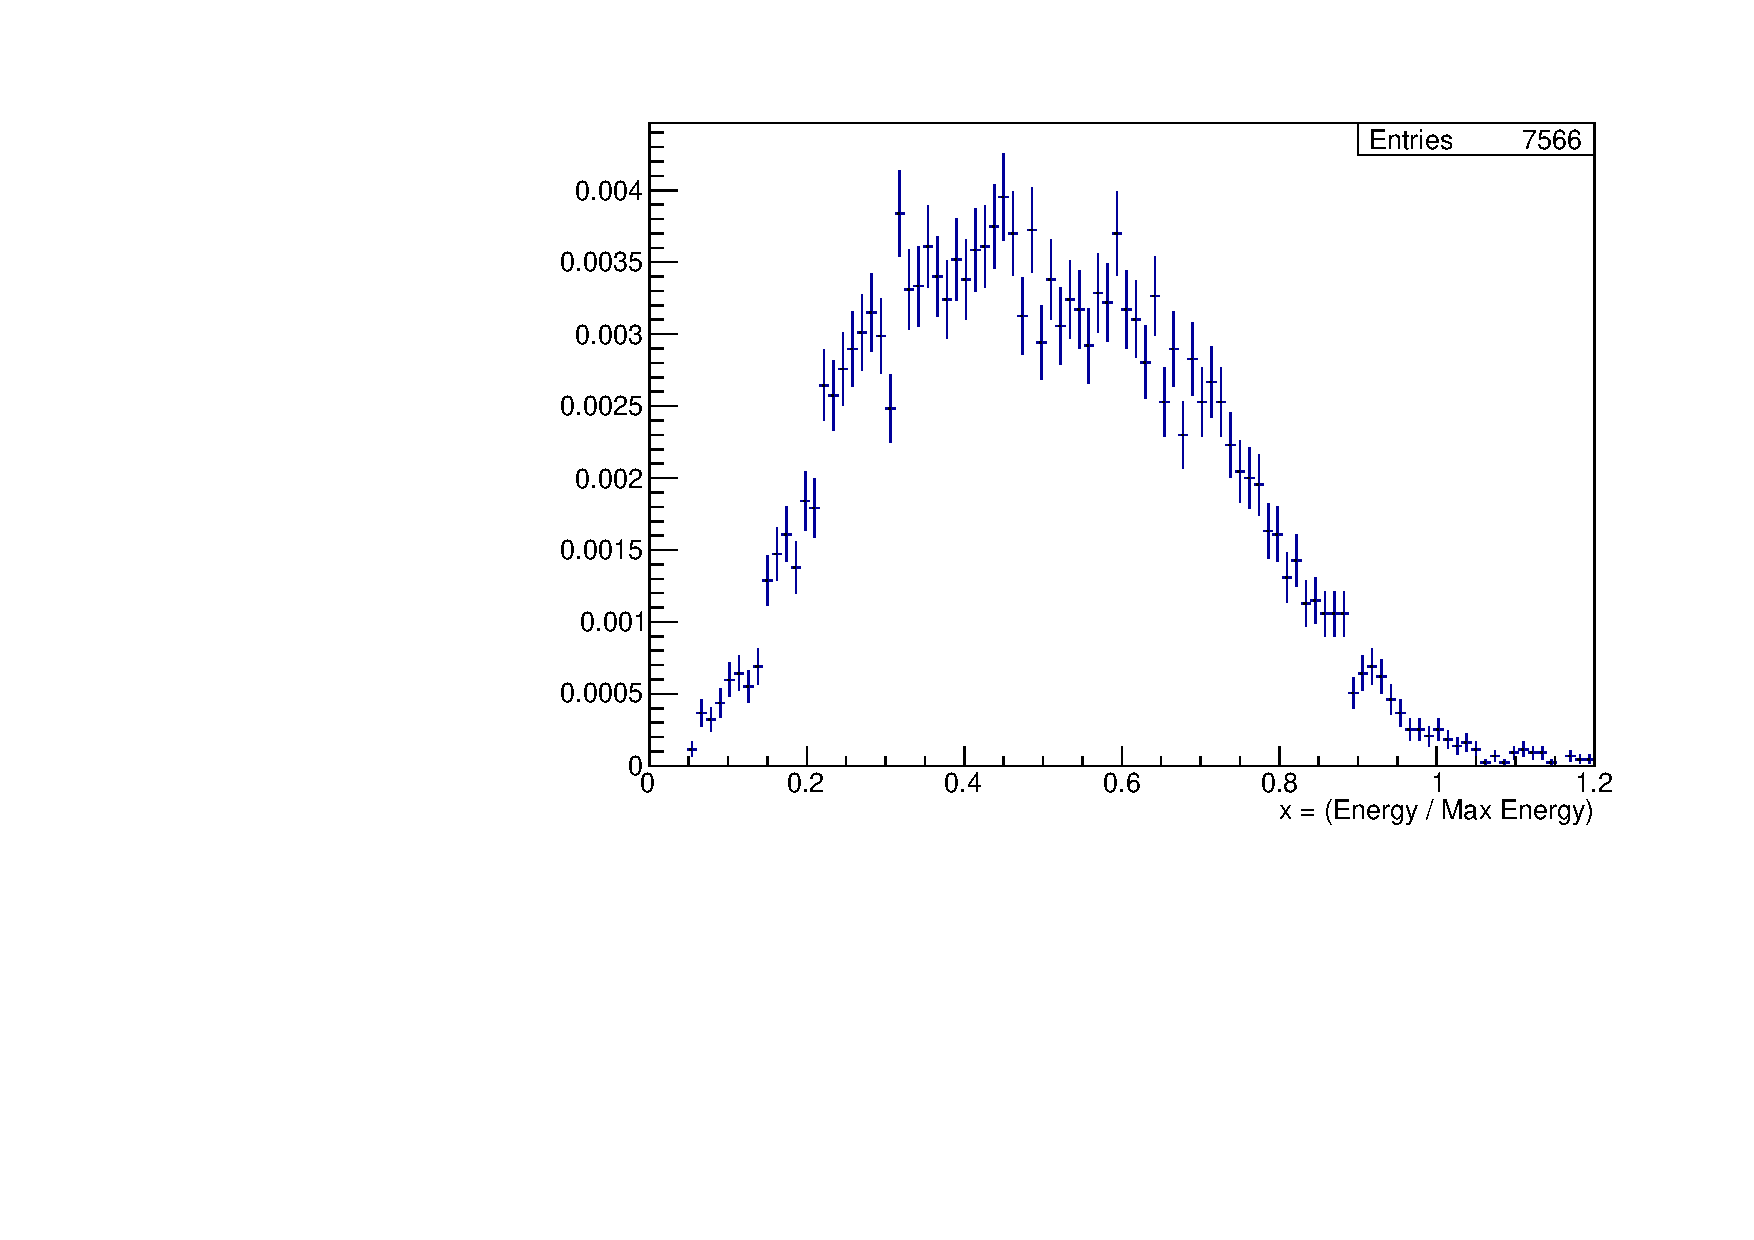
\includegraphics[height=\columnwidth,angle=-90]{figure/ikemitsu/michel_PS.pdf}
\caption{PS で得られたエネルギー分布(磁場なし標的)}
\label{michel_PS}    
\end{minipage} 
\begin{minipage}{0.4\columnwidth}
\centering
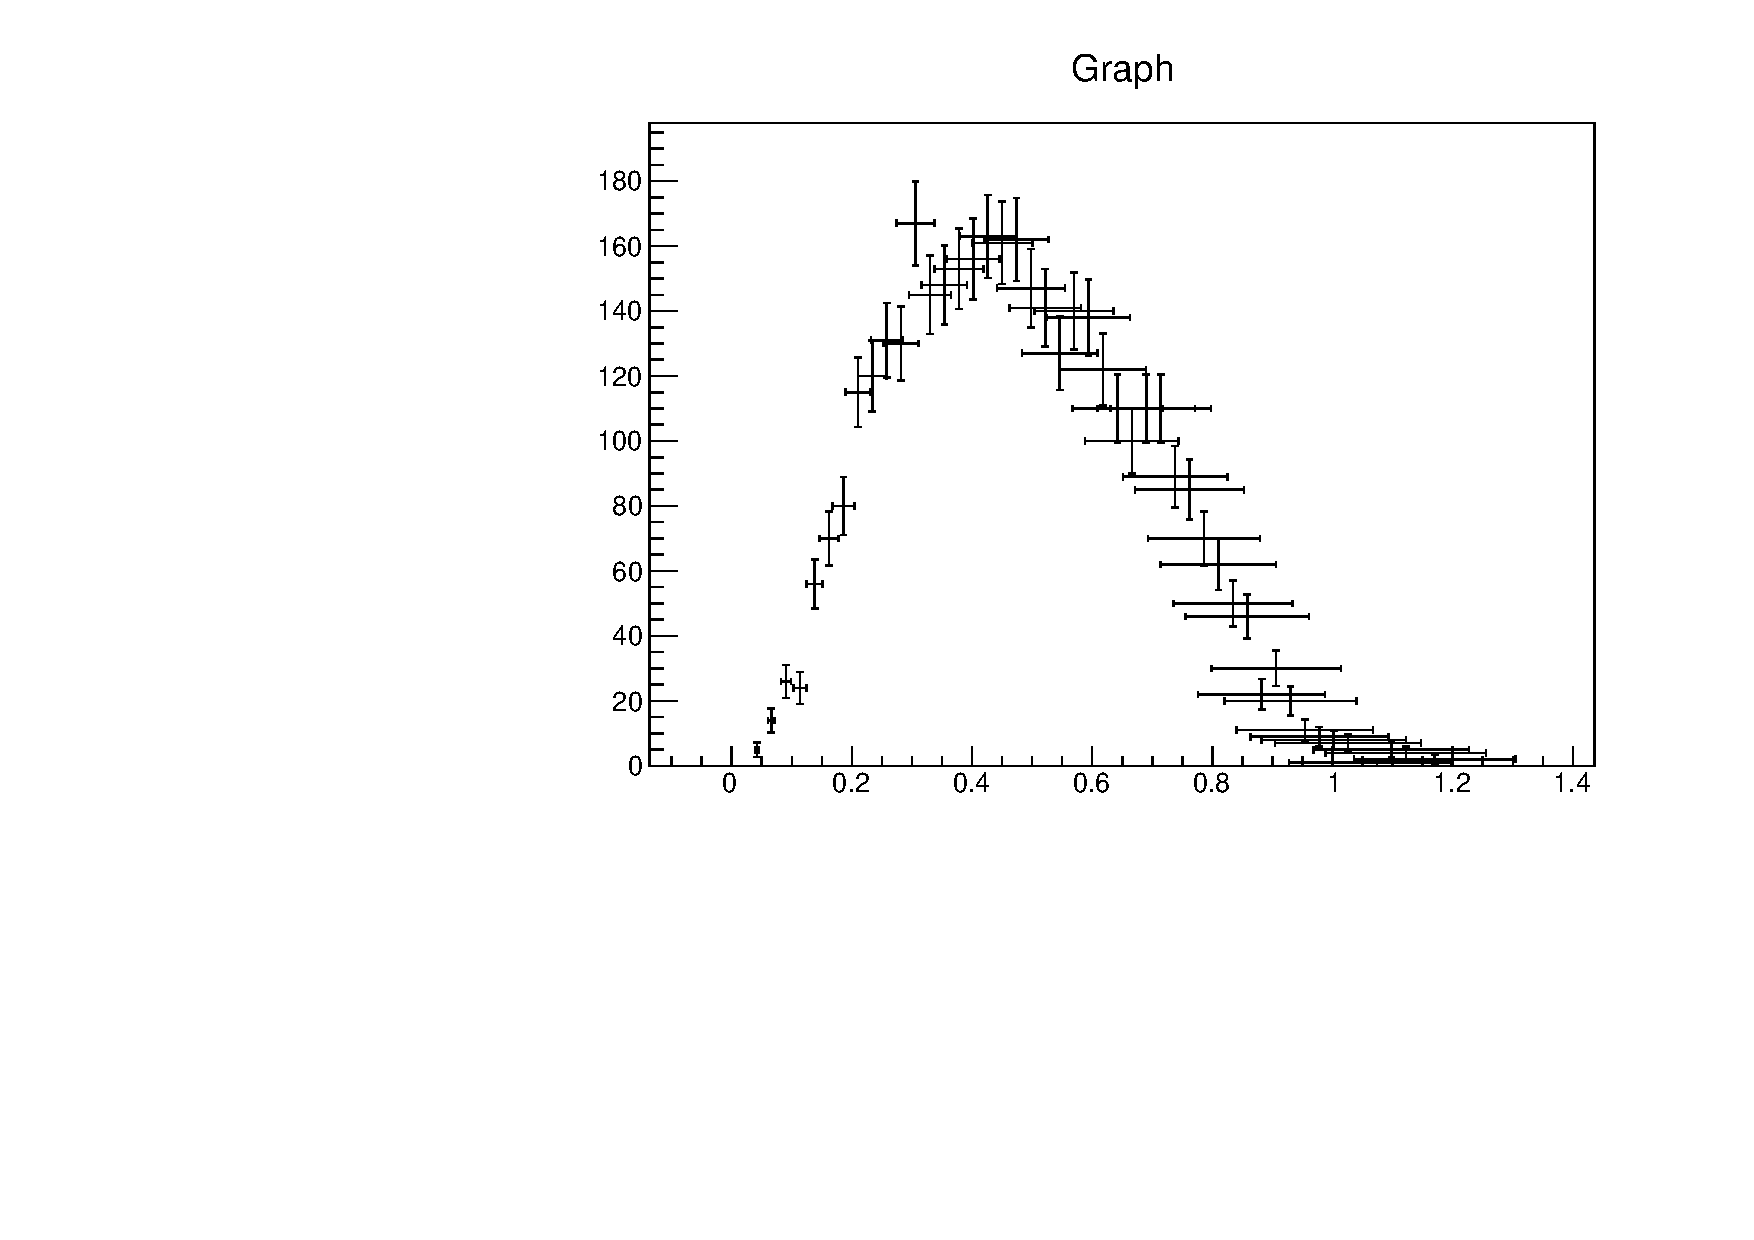
\includegraphics[height=\columnwidth,angle=-90]{figure/ikemitsu/michel_PS_gosa.pdf}
\caption{PS で得られたエネルギー分布(磁場なし標的,誤差付き)}
\label{michel_PS_gosa} 
\end{minipage}
\end{figure}
  
ミューオンのスピンに対して角度$\theta$ の方向に崩壊する$e^{+}$ のエネルギー分布は,式~\eqref{eq:theory_michel} で与えられる.この式に$\rho$ 以外のパラメータの値として,標準模型で予想されている$\eta = 0 , \;\xi = 1 , \;\xi \delta = 3/4$ を代入して計算すると,
\[\frac{d\Gamma}{dx} \propto x^{2} [\frac{2}{3}(\rho + \frac{3}{8}\cos \theta - \frac{1}{8})(4x-3) + \frac{1}{4}(\cos \theta + 3)]\]
となる.

図~\ref{michel_PS_gosa} のグラフを$f_{\mathrm{michel}}(x) = x^{2} (A(4x -3) + B)$ でフィッティングすることにより$\rho$ を求めることができると考えたがうまくいかなかった.この原因として,高エネルギー側での横軸の誤差が大きいことや検出器のエネルギー分解能を考慮せずにフィッティングを行っていることが考えられる.本解析では時間の都合上これ以上の解析は行なわなかった.

\subsubsection{エネルギー測定についての今後の課題}
以下ではエネルギー分布測定についての今後の方針を述べる.

プラスチックシンチレータは無機シンチレータに比べて密度が小さいので制動放射で生じるフォトンは少ない.したがってフォトンによるエネルギー漏れは少なく,これに起因する測定エネルギーのゆらぎは比較的小さい.しかし,シンチレーション効率が低いプラスチックシンチレータの信号をPMT で読み出すにはゲインを高くする必要があり,PMT の電子増倍過程の確率的なゆらぎによってエネルギー分解能が悪くなる.
  %PSは無機シンチレータに比べて密度が小さいので,電磁シャワーで生じたフォトンが検出器の外側に漏れやすい.%フォトンの発生の頻度がNaIに比べて低いことも注目すべき
  %これによって測定されるエネルギーが入射粒子のエネルギーよりも低くなるイベントが生じる.
  %したがって測定の結果得られるエネルギー分布は入射粒子の分布と比較して高エネルギー側が少なく低エネルギー側が多い分布になる.
  %これによって高エネルギーの粒子の観測数が減ると考えられる.%観測数とはなにか?
したがって,解析においては測定されるエネルギーにPMT 由来のゆらぎがあることを考慮する必要がある.
  %解析的にこの課題を解決するには,シミュレーションによって入射粒子のエネルギーと観測されるエネルギーの対応を求めてfitting関数にその寄与を組み込む必要がある.

具体的にはまず,エネルギー$E_\mathrm{in}$ をもつ粒子が検出器中で失うエネルギー$E_\mathrm{loss}$ の分布をシミュレーションによって求め,それを適当な関数で近似する.これを0から50~MeV の$E_\mathrm{in}$ に対して行い,$E_\mathrm{loss}$ の分布関数$f(E_\mathrm{in}, E_\mathrm{loss})$ を求める.次に,入射粒子のエネルギー分布$g_{\mathrm{real}}(E)$ を$f(E_\mathrm{in}, E_\mathrm{loss})$ でたたみ込み積分することで,損失エネルギーの分布関数$g_{\mathrm{loss}}(E)$ が得られる.最後に,PMT に起因するゆらぎの寄与として$g_{\mathrm{loss}}(E)$ をガウシアンでたたみ込み積分して,予想される測定値の分布関数$g_{\mathrm{measure}}(E)$ が得られる.得られた$g_{\mathrm{measure}}(E)$ を用いてフィッティングを行う.
  %解析的にこの課題を解決するには,シミュレーションによって入射粒子のエネルギーと観測されるエネルギーの対応を求めてfitting関数にその寄与を組み込む必要がある.%それでそれに対してどうするのか?
  
また,この実験ではプラスチックシンチレータのエネルギー較正に改善の余地が大いに残されている.一つの方法としてベータ線源の$Q$~値を求めることで較正点を増やすことができる.他に,宇宙線ミューオンを用いたキャリブレーションならば,フィンガーカウンターとのコインシデンスを取ることによって宇宙線の飛跡を制限して測定を行うことが考えられる.こうすることで測定される宇宙線の損失エネルギーの幅は図~\ref{ps_langau} よりも狭くなり,また,いくつかの飛跡に対してエネルギー測定を行うことで異なる損失エネルギーに対する電荷量を求められる.すなわち,較正点が増えて各点における誤差が小さくなると予想される.したがって,測定する宇宙線の飛跡を制限することで較正直線の誤差を小さくすることができると考えられる.
  %宇宙線ミューオンを用いたキャリブレーションならば,NaI検出器で行っているような,fingerとのcoincidenceをとることで精度を上げることができると考えられる.
  % NaIではfingerとのcoincidenceをとるといった処理はしていない.事実誤認.

  %%%%%%%%%%%%%%%%%%%%%%%%%%%%%%%%%%%%%%%%%%%%%%%%%%%%%
  %しかし,寿命に関して表~\ref{fitrange1}と表~\ref{fitrange2}の1,2段目を比較すると,遅い時間側でfittingを行うと寿命が長くなっていると分かる.
  %これは,バックグラウンドなどのノイズを信号として処理しており,その影響がイベント数の少ない部分で強く出ていることによると考えることができる.
  %これを除くためには,より詳しい波形解析によってノイズとみなせる信号の性質を特定しなければならない.
  %今回の実験ではバックグラウンド計測をしなかったが,今後の課題として,ノイズ除去を目的とした解析を行う必要がある.
  %ノイズとして想定されるものには,
  %WFDを用いた実験では波形をデータとして残せるので,こうしたノイズに起因する信号を取り除くことは可能だと考えられる.
  %寿命の解析結果として,表~\ref{fit_lt}と表~\ref{fitrange1}・表~\ref{fitrange2}の違いをfitting範囲による系統誤差に含めた.%どのように?
  %WFDを用いた実験では波形をデータとして残せるので,ノイズに起因する信号を取り除くことは可能だと考えられる.%どのようなノイズが想定されている?
  %寿命の解析結果として,表~\ref{fit_lt}と表~\ref{fitrange1}・表~\ref{fitrange2}の違いをfitting範囲による系統誤差に含めた.%どのように?

  %$g$因子については,バックグラウンドがあっても振動の周期への影響はないと考えられる.%なぜ?
  %したがって,fitting範囲による系統誤差はないとした.

  %%%%%%%%%%%%%%%%%%%池満パート終了%%%%%%%%%%%%%%%%%%%

 %\end{document}
